如图,一个边长是1厘米的等边三角形ABC,将它沿直线$l$作顺时针方向的翻动,到达图示中最右边三角形的位置.试在A、B、C三个顶点中选一个点,求该点所经过的路程是多少厘米.(精确到0.01厘米)

\begin{flushright}

    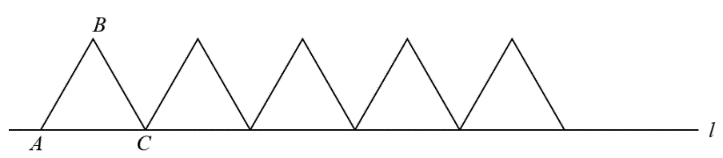
\includegraphics[height=1.5cm]{lib/image/MJA04020115.png}

\end{flushright}



